\documentclass[10pt,a4paper]{article}
\usepackage[latin1]{inputenc}
\usepackage{graphicx}
\usepackage{amsmath, amsfonts, amsthm, amssymb}
\usepackage{mathtools}

\begin{document}
\begin{center}
\Huge{Project plan}\\[.2cm]
\Large{A Graphical User Interface (GUI) for weather radar and wind energy data visualization and analysis}\\[.2cm]
2nd version. March 2012
\end{center}
\textbf{Group 5.1}\\
Mads Engel Lundt, s103439\\
Matthias S. Alan Larsen, s103437\\
Joachim Vestmark Vith Jensen, s103430\\

\section{Analysis}
From the project description on CampusNet:

"\emph{Background: Wind energy applications such as wind power prediction require the use of large amounts of data. These data come from multiple sources (e.g. onsite observations from measuring stations, meteorological forecasts from Numerical Weather Prediction models, images from weather radars) and, consequently, have very diverse formats (times series, georeferenced data, gridded data). This raises an important issue since there does not exist any common or efficient platform for their visualization and analysis.}

\emph{The objective is to design a user-friendly GUI for enhancing the combined visualization of several sources of data. The following initial specifications will serve as a starting point for the project: }
\begin{itemize}
\item \emph{efficient system for data request, retrieval and display}
\item \emph{handling of animations (it is crucial as most data consist of  time series or of series of images)}
\item \emph{preferences should be given to open source softwares/programming languages/solutions}
\item \emph{operationability of the final GUI on web browsers will be considered}
\end{itemize} 
"

\newpage

\section{Solution strategy}
Based on the analysis of the project, our solution will be solely webbased using an interactive map with several data layers shown in an intuitive way.\\
We have chosen to implement a database in the solution, as it would make the application much faster if specific data only should be processed once, where after it can be fetched from the database.\\
OpenStreetMap will be used for the map data. The following technologies will also be used:\\
\begin{itemize}
  \item PHP
  \item C/C++
  \item JS
  \item HTML/CSS
\end{itemize}
Using the following frameworks will ease the workload and make the application more flexible:\\
\begin{itemize}
  \item Qt
  \item FuelPHP
  \item jQuery (including flot and Leaflet)
\end{itemize}
A Block Diagram of the application is below. The point is that an administrator uploads a data file that will be processed and the data saved. When a person uses the application, saved data will then be shown to him.
\begin{figure}[!ht]
\centering
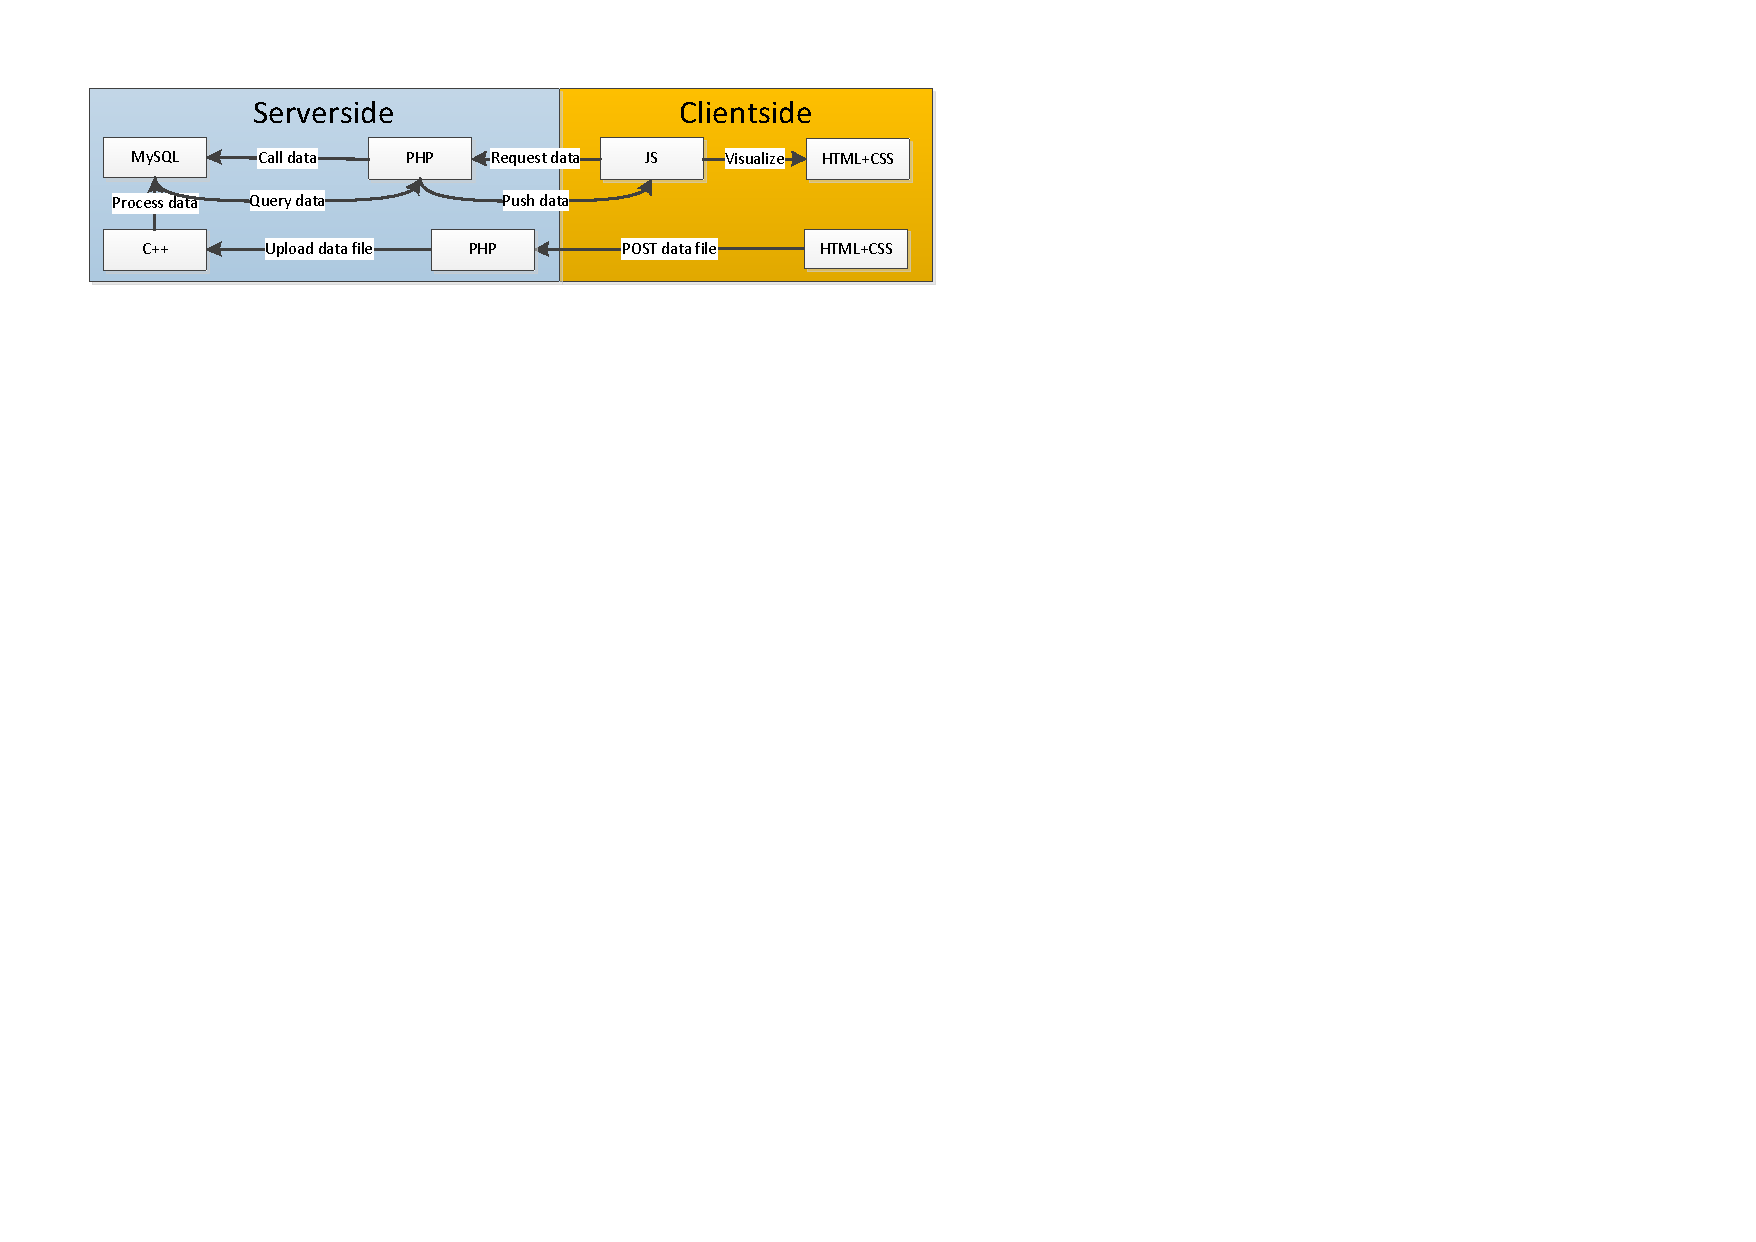
\includegraphics[bb=1cm 16cm 16cm 20cm,scale=0.9]{blockdiagram}
\caption{Block Diagram}
\end{figure}

\newpage

\section{Time schedule}

\begin{figure}[!ht]
\centering
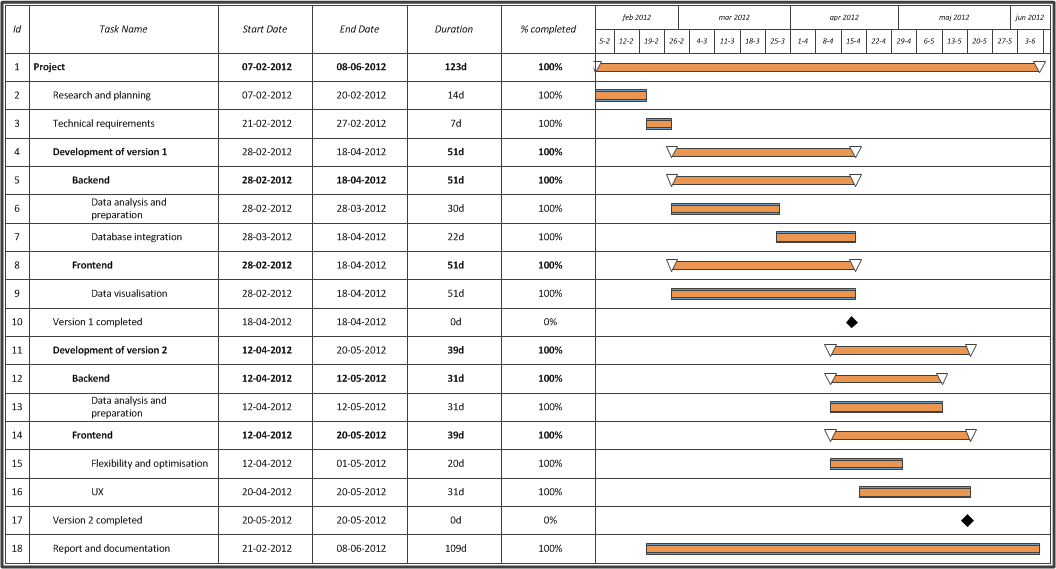
\includegraphics[bb=1cm 28cm 18cm 28cm,scale=0.8]{planning2}
\end{figure}
\newpage

\section{Work distribution}

As seen on the time schedule, we have split the application into two versions. For version 1, the work distribution is as follows:
\begin{itemize}
  \item C++ and database creation: Matthias
  \item PHP: Joachim
  \item HTML/CSS/JS: Mads
\end{itemize}

\end{document}